\documentclass{article}

% packages and configurations
\usepackage{hyperref}
\usepackage{animate} % needed for animations and videos
\usepackage{bm} % bold font in equation environments
\usepackage[utf8]{inputenc}	% für Umlaute ect.
\usepackage{fancyhdr} % für header
\usepackage{lastpage} % für footer
\usepackage{extramarks} % für header und footer
\usepackage{amsthm} % math stuff
\usepackage{amsmath} % math stuff
\usepackage{amssymb} % math stuff
\usepackage{color}
\usepackage{listings} % code listings
\usepackage{graphicx} % für graphics
\usepackage[toc]{glossaries} % Glossar
\usepackage{color}
\usepackage{tikz}
\usepackage[absolute,overlay]{textpos} %to translate graphics through space
\usepackage{soul}
\usepackage{xcolor}
\usepackage{textpos}
\usepackage{caption}
\usepackage{parcolumns}
\usepackage{enumerate}
\usepackage[ngerman]{babel} % Umlaute
\usepackage[T1]{fontenc}    % this is needed for correct output of umlauts in pd
\usepackage[section]{placeins} %forces placeins to stay in section
\usepackage{datetime} % custom dates
\usepackage{afterpage}
\usepackage[section]{placeins}


\title{Bringing together visual analytics and probabilistic programming languages}
\author{Jonas Aaron Gütter  \\
	Friedrich Schiller Universität Jena  \\
    Matrikelnr 152127 \\
    Prof.Dr. Joachim Giesen \\
    M. Sc. Phillip Lucas
	}

\makeglossaries


\begin{document}


\maketitle

\begin{abstract}
A probabilistic programming language (PPL) provides methods to represent a probabilistic model by using the full power of a general purpose programming language. Thereby it is possible to specify complex models with a comparatively low amount of code. With Uber, Microsoft and DARPA focusing research efforts towards this area, PPLs are likely to play an important role in science and industry in the near future.
However in most cases, models built by PPLs lack appropriate ways to be properly visualized, although visualization is an important first step in detecting errors and assessing the overall fitness of a model. This could be resolved by the software Lumen, developed by Philipp Lucas, which provides several visualization methods for statistical models. PPLs are not yet supported by Lumen, and the goal of the master thesis at hand is to change that by implementing an interface between Lumen and a chosen PPL, so that exploring PPL models by visual analytics becomes possible.
The thesis will be divided into two main parts, the first part being an overview about how PPLs work and what existing PPLs there are available. Out of these, the most appropriate one will be chosen for the task. The second, more practical part will then document the actual implementation of the interface.

\end{abstract}

\tableofcontents

\newglossaryentry{Bayesian network}
{
  name=Bayesian network,
  description={...}
}

\newglossaryentry{conditional probability distribution}
{
  name=conditional probability distribution,
  description={...}
}

\newglossaryentry{inference algorithm}
{
  name=inference algorithm,
  description={is a key part of a \gls{probabilistic reasoning system}}
}

\newglossaryentry{joint probability distribution}
{
  name=joint probability distribution,
  description={...}
}

\newglossaryentry{marginal distribution}
{
  name=marginal distribution,
  description={...}
}

\newglossaryentry{probabilistic model}
{
  name=probabilistic model,
  description={is a key part of a \gls{probabilistic reasoning system}}
}

\newglossaryentry{probabilistic programming}
{
  name=probabilistic programming,
  description={is something}
}

\newglossaryentry{probabilistic programming language}
{
  name=probabilistic programming language,
  description={is used to create a \gls{probabilistic reasoning system} more effectively than with a conventional programming language}
}

\newglossaryentry{probabilistic reasoning system}
{
  name=probabilistic reasoning system,
  description={consists of a \gls{probabilistic model} and an \gls{inference algorithm}}
}

\newglossaryentry{Turing-complete}
{
  name=Turing-complete,
  description={a turing-complete machine can perform any computation that could theoretically performed by any computer. universally programmable.}
}
\printglossaries
\section{Road Map}

\begin{enumerate}
	\item Getting started
	\begin{itemize}
		\item set up Master thesis document
		\item Probabilistic Programming Languages
		\begin{itemize}
			\item play at least with: PyMC3, Stan
			\item read the docs, wiki, ...
			\item download the libraries
			\item reproduce the getting started tutorials
			\item --> understand the ideas and how to use it, get a feeling for it
		\end{itemize}
		\item theoretic background: Read Bayesian Data Analysis part I, Chapter 1,2 and part II, chapter 6,7
		\item Lumen
		\begin{itemize}
			\item install locally and play with
			\item understand main idea of Lumen and what we want to do with it
		\end{itemize}
		\item Start filling up your MA thesis document
		\begin{itemize}
			\item understand and write down in MA thesis the "why \& what"
			\item describe the background of the work, e.g. summarize PPLs
		\end{itemize}
		\item give a short presentation
		\begin{itemize}
			\item what have you done and learned
			\item what do you plan to do?
			\item why is it relevant?
			\item how do you plan to measure the success?
		\end{itemize}	
	\end{itemize}
	\item First connection of PPLs to Lumen
	\begin{itemize}
		\item Start from small, very simple and specific example. Generalize later.
		\item Choose PPL to work with
		\begin {itemize}
		\item work out requirements on PPL
		\item work out preferred features of PPL
		\item choose a PPL based on these requrements and preferences
	\end{itemize}
	\item design wrapper of PPL with Lumen
	\begin{itemize}
		\item work out requirement and interface
		\item identify necessary work on Lumen
		\item identify necessary work
	\end{itemize}
	\item Connect chosen specific example with lumen
	\item Continue to work on your master thesis document!
\end{itemize}
\item Improve, generalize and clean up the connection of your PPL to Lumen
\end{enumerate}

\section{Rules of Probabilistic Inference}

There are three rules of probabilistic inference: The chain rule, the total probability rule, and the Bayes' rule. The following explanations are taken from \cite{9781617292330}.

\subsection{Chain rule}

The chain rule is used to calculate a \gls{joint probability distribution} of several variables from local \gls{conditional probability distribution}s of these variables:

\begin{equation}
  P(X_1 ,X_2 ,...X_n ) = P(X_1 )P(X_2 | X_1 )P(X_3 | X_1 ,X_2 )...P(X_n | X_1 ,X_2 ,...X_{n-1}) )
\end{equation}

\subsection{Total probability rule}

The total probability rule calculates the probability distribution over a subset of variables, also called a \gls{marginal distribution}, by summing out all the other variables, that is by summing the probability distributions for each combination of values of these variables:

\begin{equation}
P(\boldsymbol X |\boldsymbol Z ) = \sum_{\boldsymbol y}   P(\boldsymbol X ,\boldsymbol Y =\boldsymbol y |\boldsymbol Z )
\end{equation} 

\subsection{Bayes' rule}

Bayes' rule calculates the probability of a cause, given aneffect, by using the prior probability of the cause and the probability of the effect, given the cause. The Bayes' rule can be derived from the chain rule.

\begin{equation}
P(X|Y) = ( P(Y|X) * P(X) ) / P(Y)
\end{equation}

\section{Bayesian models}

According to \cite{1439840954}, there are 3 basic steps in Bayesian data analysis: Setting up a joint probability model, calculating a posterior distribution, and assessing the model performance

"Classical" approach: Evaluate the procedure used to estimate the parameters over the distribution of possible outcome values conditional on the true unknown parameters.

Bayesian approach: Estimate the parameters conditioned on the outcomes.

Bayesian models are about finding a full probability model for a given problem, whereas conventional models only deal with estimation of the most likely parameters.
The model parameters $\beta$ themselves are also considered as random variables which depend on hyperparameters $\alpha$.
\\
According to \cite{Wang2018}, the likelihood of a new datapoint can be calculated by integrating the product of the prior likelihood and conditional probability of $\beta$ over the space of $\beta$, as shown in equation \ref{eq:posterior_predictive}. This formula can also be derived using the chain rule (I think).



\begin{equation}
p(x_{new}|\boldsymbol x, \alpha) = \int p(x_{new}|\beta) * p(\beta | \boldsymbol x,\alpha) d \beta
\label{eq:posterior_predictive}
\end{equation}



\section{What is Probabilistic Programming}

Modelle spezifizieren/beschreiben 

\cite{wiki:Probabilisticprogramminglanguage}

effizienter in der Beschreibung von Modellen als herkömmliche Programmiersprachen \cite{Hardesty2015}

unifying general purpose programming with probabilistic modeling \cite{probabilistic-programming.org}


A \gls{probabilistic reasoning system} uses prior knowledge in the form of a \gls{probabilistic model} to answer a certain query. The particular propertes of the query as well as the prior knowledge are given to an \gls{inference algorithm} which returns an answer in the form of probabilities. Example is shown in figure \ref{fig:example_prs}. Probabilistic Programming is the implementation of a \gls{probabilistic reasoning system} by using a programming language.

Traditional means for representing models are not always sufficient for probabilistic models. Therefore, probabilistic programming languages were introduced to be able to represent models with the full power of a programming language (http://www.probabilistic-programming.org/wiki/Home).


\begin{figure}
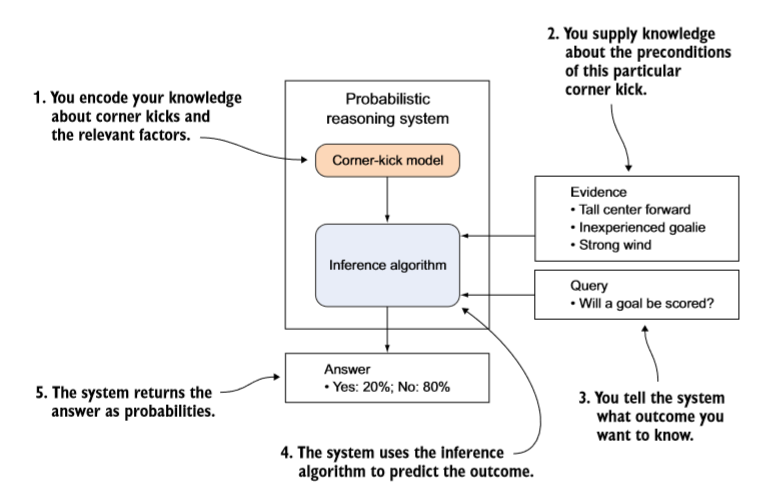
\includegraphics[width=\textwidth]{images/probabilistic_reasoning_system.PNG}
\caption[General workflow example of a probabilistic reasoning system. Source: \cite{9781617292330}]{General workflow example of a probabilistic reasoning system}
\label{fig:example_prs}
\end{figure}

% how to call a glossar entry: 

\section{Existing PPLs}

\begin{itemize}
     \item stan for python: https://pystan.readthedocs.io/en/latest/
    \item pymc3: https://docs.pymc.io/notebooks/getting\_started.html\#Case-study-2:-Coal-mining-disasters
    \item edward: http://edwardlib.org/getting-started
    \item pyro: http://pyro.ai/
\end{itemize}

\subsection{Stan for python}

transformed parameters are parameters which depend on hyperparameters.

\subsection{Pymc3}

python library

fit Bayesian models, including Markov Chai Monte Carlo (MCMC) and variational inference (VI)


\subsection{Edward}

\subsection{Pyro}


\section{Lumen}

\listoffigures
        
\section{Literatur}

\bibliography{Literatur.bib}
\bibliographystyle{ieeetr}


\end{document}